
% summary of this section.
In this section we report on the development and verification of a complex model
translation\markus{transformation?} that is used to compile high level embedded
system models to C programs. We start with some background on mbeddr the
language and infrastructure used to express the high level embedded software
models. We then highlight the importance of this case study has for embedded
software in safety-critical systems, and how SyVolt can contribute to the
development of these.

Then we give an overview of the translation that performs the compilation of
mbeddr models and we show an example contract that a correct compilation must
satisfy. We end the section with some discussion about the limits of the SyVolt
contract language\markus{Should this discussion be part of the CS? Or more
generally part of a general discussion section?}.

\subsection{mbeddr: Extensible Languages for Embedded Software}

% What is mbeddr and what it is used for.
mbeddr\cite{Voelter:2012:MEC:2384716.2384767} is a set of domain-specific and
general-purpose languages for embedded software development. While it also
provides support for process aspects and formal verification, it's core is a set
of extensions to the C programming language specific to the domain of embeded
software development. These extensions provide first-class language support for
well-known abstractions for programming embedded systems. Examples include
decision tables, components and interfaces, state machines or physical units.
mbeddr is open source software and has been used both academically and in
industry~\cite{Voelter2013,Voelter2014,mry_et_al:DR:2014:454,mbeddrSM}. mbeddr
relies on the JetBrains MPS language workbench\markus{ref} to enable flexible and modular
language extensibility.

% Components
Components are a useful abstraction because support modularization of
functionality as well as the separation of implementation and specification.
mbeddr allows the developer to declare interfaces, each with a set of operation
signatures (\emph{specification}). Components then declare provided or required
ports. Each port is associated with an interface; if a component provides a
port, it must implement the operations declared in the interface of that port
(\emph{implementation}). Instances of components communicate between each other
by invocating operations through their required ports. These instances of
components are ``wired together'' by specifying, for each required port, what
provided port -- and by extension the component instance that provides that port
-- satisfies that requirement.
The implementation of operations can be done with pure C code, decision tables,
state machines or any DSL developed with MPS.

\markus{Remove dec tables and state machines? Not relevant for CS.}
% Decision tables
Decision tables essentially abstract nested if statements. They are a useful abstraction because one can quickly express decision making based on a large number of variables. 

% State machines
State machines abstract switch/case statements. mbeddr also provides special syntactic constructs that allow the state machine to interact with its surrounding code, for instance, react to a invocation coming through a provided port. In mbeddr, state machines can only access local variables.

% Simple example and disclaimer that the simple example is not the case study.
To illustrate mbeddr, we show a simple example but please notice that this
example is not the case study\markus{Why not? How is the CS different?}.
The case study is the compilation of any mbeddr model to C\markus{Not really.
You only deal with components, right? Not the rest of mbeddr.} and not just this
simple example.
Listing~\ref{code:simple_example_mbeddr} shows the textual
syntax\footnote{C, interfaces and components use a textual notation in MPS.
However, as a consequence of MPS' projectional editor, users can also use other
notations such as tables, math or diagrams. While these other notations are
heavily used in mbeddr, they are not relevant to this case study} of the mbeddr
model.


\lstset{language=C, caption={Client/Server Example in mbeddr},
label=code:simple_example_mbeddr, morekeywords={exported, cs, interface, void,
string, provides, requires, components, op, return,instance, connect,
to, instances, int32}} 
\begin{lstlisting}[float] 
exported cs interface Client { 
  void client_process() 
} 

exported cs interface Server { 
  string server_process(string request) 
} 

exported component Client { 
  provides Client clientInterface 
  requires Server clientcomp_serverInterface 
   
  void clientInterface_client_process() <= op clientInterface.client_process { 
    clientcomp_serverInterface.server_process("Hello"); 
  }  
}  

exported component GoodServer { 
  provides Server serverInterface 
  string serverInterface_server_process(string request) <= op serverInterface.server_process { 
    return request; 
  }  
}  

exported component BadServer  { 
  provides Server serverInterface 
  string serverInterface_server_process(string request) <= op serverInterface.server_process { 
    int32 x = 0; 
    while (x >= 0) { 
      x = x + 1; 
    } 
    return request; 
  } 
} 

instances inst { 
  instance ClientComponent clientComponent 
  instance GoodServer gserverComponent 
  instance BadServer bserverComponent 
  connect clientComponent.clientcomp_serverInterface 
       to gserverComponent.serverInterface
}
\end{lstlisting}

\markus{Instead of using quotation marks below, you should urgently introduce
code font for identifiers in the text!}

This example consists of two interfaces, three components and one instance of
each component:
\begin{compactdesc}
\item[Client and qServer interfaces] define the operation signatures akin to how
function prototypes are defined in C.

\item[Client component] provides the Client interface through a port called
``clientInterface'' and requires the Server interface through a port called
``clientcomp\_serverInterface''. The implementation of the operation
``client\_process'', declared in the Client interface is just the invocation of
the ``server\_process'' operation of the Server interface through the
``clientcomp\_serverInterface'' port.

\item[GoodServer component] provides the Server interface and the implementation
of the ``server\_process'' operation is just an echo.

\item[BadServer component] provides the Server interface and the implementation
of the ``server\_process'' operation is an infinite loop. The reason for this
odd choice off example will become clear in the next section.

\item[Instances] are declared for each component and the required
``clientcomp\_serverInterface'' port of the Client component instance is
connected to the provided ``serverInterface'' port of the GoodServer component
instance.
\end{compactdesc}


\subsection{Correct Embedded Systems}

% Embedded systems need to be reliable.
The main reason for us to choose this case study is that embedded systems need
to be reliable: there are industry standards such as ISO-26262, DO-178B or
IEC-61508 to help ensure reliability and there are critical embedded systems
such as pacemakers \cite{mry_et_al:DR:2014:4543} that must be shown to be
correct.

% Traditional development of reliable embedded systems
Traditionally, embedded systems are implemented in C code and reliability is
ensured by a combination of testing and formal verification techniques such as
model checking. However, testing only guarantees reliability in as far as the
test cases go, and achieving the necessary high coverage is a lot of work.
Model checking, on the other hand, is very expensive because of C's high
expressivity and the resulting state space explosion problem. In order to
properly apply model checking techniques \cite{Ivancic2005}.
The abstraction process is error prone and time consuming as is described in
\cite{Corbett2000} and \cite{Ratiu:2012:LEE:2663689.2663692}.

% Mbeddr contribution to the reliable embedded systems development
mbeddr represents an evolution of traditional embedded system development
because it starts with abstractions that can be proven to be
correct\markus{That's probably a bit strong. Let's discuss how to say this
better} and then generates C code.
Model checking techniques can be applied to mbeddr models because they contain
higher level information (e.g., state machines, decision tables or contracts on
interface) whereas with plain C code, these abstractions need to be inferred
from the C.

% how does mbeddr help ensure correct embedded systems
\markus{This is no longer true. We use Sat4J and CBMC.}
% mbeddr is integrated with the NuSMV~\cite{Cimatti2002} model checker to perform
% model checking of the state machines and with the Yices~\cite{Dutertre:cav2014}
% Satisfiability Modulo Theories (SMT) solver to check the consistency and
% completeness of the decision tables.

% properties vs contracts
It is important to distinguish two types of properties: properties that a given
mbeddr model needs to satisfy; and properties that all mbeddr models need to
satisfy. For instance, a property of the former type for the mbeddr model of the
pacemaker system is that it never stops. A property of the later type is that
decision tables, if they are used, must be consistent and
complete~\cite{Ratiu:2012:LEE:2663689.2663692} or that contracts expressed on
interfaces are fulfilled by all implementing components.

% the problems with mbeddr level of abstraction
As described in~\cite{Ratiu:2012:LEE:2663689.2663692}, properties checked at the
mbeddr level can only be sound if the C code that is generated satisfies the
same properties as the mbeddr models. It is this crucial to achieve soundness of
the transformations from mbeddr's abstractions down to C. In practice this
correctness is ensured by manual reviews of the code generation and
lots of automated tests.

% how can syvolt help to ensure reliability
SyVolt is a step towards ensuring the C code generation is \emph{always}
correct, provided the appropriate correctness properties (of the C code
generation) are described. SyVolt allows the the transformation developer to
express contracts that relate the generated C construct to the constructs
available as extensions. This is something that cannot be done by checking the
generated C code alone as it requires the traceability information between the
generated C code and the mbeddr model\markus{This last sentence seems oddly
out of place. Why is this trace stuff relevant here?}.

% example
\markus{Is this merely an example, or is this THE CASE STUDY? I thiink the
latter. Rephrase?} For instance, in SyVolt it is possible to prove that the
wiring of instances of components is always translated to C correctly, i.e.,
when executing the C code, no instance will invoke a different operation than
the one that is specified in the wiring scheme at the mbeddr components level.
This is an important contract as it ensures, for instance, that the Client
component instance in our Client/Server example (see
Listing~\ref{code:simple_example_mbeddr}) will never invoke the operation of the
BadServer component instance.

To see how non-trivial this contract can be, look at the wiring function
\verb=client_wire= of the generated code from the Client/Server example shown in
Listing~\ref{code:components_sample_c}: the wiring in the C code is done by
assignment the address of the required port operation to a function pointer that
is part of the instance's runtime data.\cgg{I must stress this complexity by
explaining better how the wriring is done and how the function is then called.
Relying on the reader to understand this complexity from the example is
non-sense.}\markus{In particular, it is important to explain WHY the pointer
indirection is used: to support polymorphism} For more complex examples, this
becomes very difficult to inspect in the generated code\markus{But we don't
verify because it is hard to inspect, because after all, we can simply run a
test. We verify because we want a Proof!}.

\lstset{language=C, caption={Client/Server Example in mbeddr},label=code:components_sample_c} 
\begin{lstlisting}[float]
struct Client_i_t {
  void (*client_process)(void*);
};
struct Server_i_t {
  char* (*server_process)(char*,void*);
};

struct Client_c_t {
  void *client_serverI_port;
  Server_i_t *client_serverI_ops;
};
struct BadServer__cdata { uint8_t aMember; };
struct GoodServer__cdata { uint8_t aMember; };

static Server_i_t bserver_serverI_ops;
static Client_i_t client_clientI_ops;
static Server_i_t gserver_serverI_ops;

static BadServer_c_t bserver_inst;
static Client_c_t client_inst;
static GoodServer_c_t gserver_inst;

char* BadServer_serverI_server_process(char *request, void *_id) 
{
  BadServer_c_t *cid = ((BadServer_c_t *)(_id));
  int32_t x = 0;
  while (x >= 0){
    x = x + 1;
  }
  return request;
}

void Client_clientI_client_process(void *_id) 
{
  Client_c_t *cid = ((Client_c_t *)(_id));
  (*cid->client_serverI_ops->server_process)("Hello",cid->client_serverI_port);
}

char* GoodServer_serverI_server_process(char *request, void *_id) 
{
  GoodServer_c_t *cid = ((GoodServer_c_t *)(_id));
  return request;
}

static void init(void) 
{
  client_wire();
  gserver_wire();
  bserver_wire();
}

static inline void bserver_wire(void) 
{
  bserver_serverI_ops.server_process = &BadServer_serverI_server_process;
}
static inline void client_wire(void) 
{_
  client_clientI_ops.client_process = &Client_clientI_client_process;
  client_inst.client_serverI_port = &gserver_inst;
  client_inst.client_serverI_ops = &gserver_serverI_ops;
}
static inline void gserver_wire(void) 
{
  gserver_serverI_ops.server_process = &GoodServer_serverI_server_process;
}
\end{lstlisting}


\subsection{mbeddr to C Code Generation}

% small intro to this section
Listing~\ref{code:components_sample_c} shows the generated C code
for the Client/Server mbeddr model shown in
Listing~\ref{code:simple_example_mbeddr}. However, we have not discussed how, in
general, is the C code generated from an mbeddr model.
The C code is generated with a model transformation specified between two
metamodels: the source metamodel is the metamodel of mbeddr's components
extension and the target metamodel is the abstract syntax of C.
\markus{This subsection here is too short, and somehow not satisfying}

\subsubsection{Source and Target Metamodels}

\markus{Somewhere we must say that these metamodels have been manually moved
over into the Syvolt world. Similarly with the trafos.}

We present a simplified version of mbeddr's components metamodel in
Figure~\ref{fig:Moduleclassdiagram}:
\begin{compactdesc}
	
\item[ImplementationModule] represents the root container of mbeddr C models.
It is composed of InstanceConfigurations, AtomicComponents and
ClientServerInterfaces. 
	
\item[ClientServerInterface] represents a set of Operations. An Operation
represents a signature, with typed arguments and a return type.
We omit these details for simplicity. In
Listing~\ref{code:simple_example_mbeddr} there are two ClientServerInterfaces --
Client and Server -- each with one Operation.

\markus{Aha, so here we have code font. We should use it consistently in the
paper for identifiers form the code.}
\item[AtomicComponent] represents a component. It has Ports, which can be
ProvidedPorts or RequiredPorts, and Runnables. Runnables essentially represent
an operation implementation. OperationTriggers define which port and operation
the runnable is implementing. In Listing~\ref{code:simple_example_mbeddr}, the
GoodServer component has one provided port, named \verb=serverInterface=, and
one runnable named \verb=serverInterface_server_process= that is executed
whenever the operation \verb=server_process= is invoked through the port
\verb=serverInterface=. We have omitted the body of the runnable.
	
\item[InstanceConfiguration] represent the runtime configuration of the
component instances. It is comprised of ComponentIntance declarations and
AssemblyConnectors. AssemblyConnectors allow the modeller to establish the
connections between required and provided ports, and the instances.  In
Listing~\ref{code:simple_example_mbeddr}, the InstanceConfiguration has three
instances and one AssemblyConnector that connects the RequiredPort
\verb=clientcomp_serverInterface= of the \verb=clientComponent= instance to the
ProvidedPort \verb=serverInterface= of the \verb=gserverComponent= instance.
This means that, the required port invocation \verb=server_process("Hello")= in
the \verb=Client= will be handled by the \verb=GoodServer=.

\end{compactdesc}

\begin{figure}
\begin{center}
  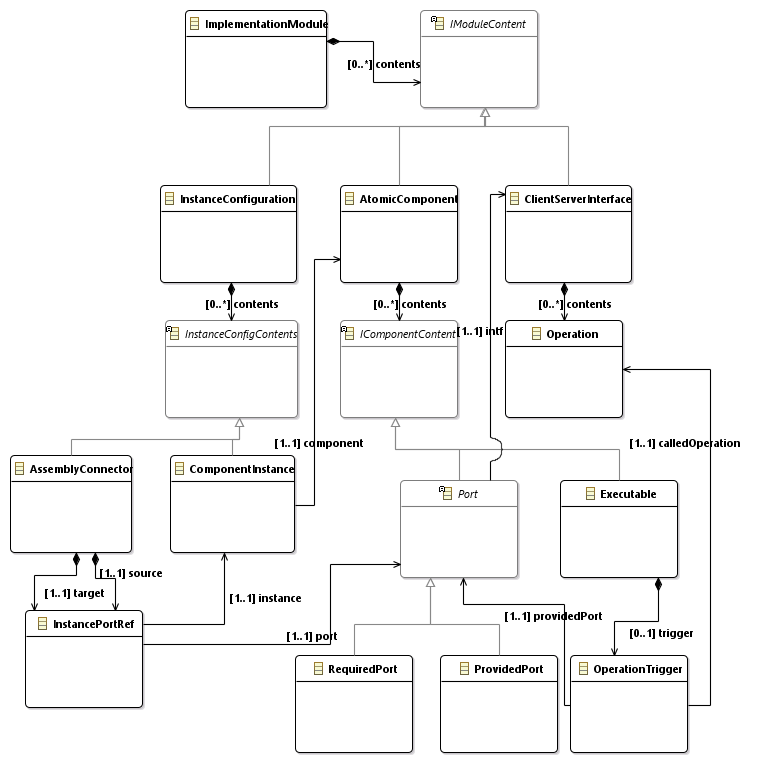
\includegraphics[width=0.48\textwidth]{figures/Moduleclassdiagram}
  \caption{Simplified mbeddr metamodel. \cgg{This picture needs to be compressed.}}
  \label{fig:Moduleclassdiagram}
\end{center}
\end{figure}

The simplified version of the C metamodel is shown in
Figure~\ref{fig:CModelclassdiagram}.
We have included only the concepts that are relevant for the contract we prove
in this case study.
A C model has multiple compilation units, which we call
ImplementationModules\markus{You've already introduced them above, but slightly
differently}.
An ImplementationModule can contain all the top-level C constructs, among them
TypeDefs, StructDeclarations, FunctionPrototypes, Functions and
GlobalVariableDeclarations.
In Listing~\ref{code:components_sample_c}, the ImplementationModule has five
StructDeclarations, six GlobalVariableDeclarations and seven Functions.
The \verb=Client_i_t= structure has a CFunctionPointerStructMember named
\verb=client_process=. The remaining concepts should be familiar to the
reader\cgg{Should I give more details about the C or can I assume that they know
C?}.\markus{Let's assume basic familiarity with C.}

\begin{figure}
\begin{center}
  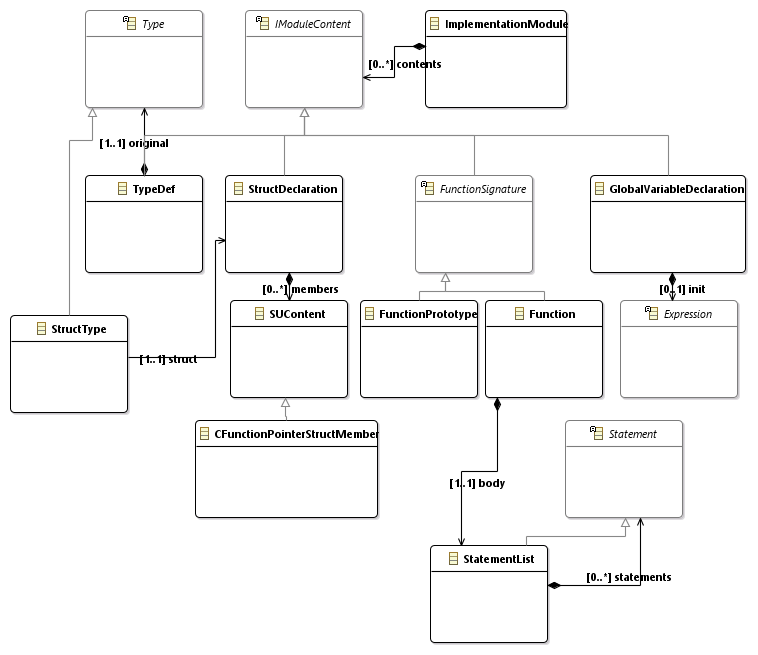
\includegraphics[width=0.48\textwidth]{figures/CModelclassdiagram}
  \caption{Simplified C metamodel. \cgg{This picture needs to be compressed.}}
  \label{fig:CModelclassdiagram}
\end{center}
\end{figure}


\subsubsection{Transformations in mbeddr}

% Why did we not use the default C code generator and disclaimer
The transformation from mbeddr's extensions to C constructs is done as model
transformations on the graphs that represent the program (based on the used
languages' metamoels). MPS comes with a language to specifiy such
transformations; it uses the concrete syntax of the target language as part of
the description of the transformation, and thus looks similar to template
languages known from regular text-generators (even though it actually describes
model transformations). Unfortunately, we are not able to apply our proof
technique\markus{Just a reminder: I assume that future work includes that we may
want to add DSLTrans into MPS?} to MPS' transformation language because of its
expressivity. Instead, we created a DSLTrans transformation that performs the
same task as the generator and in this case study we demonstrate that that
transformation is correct with respect to the contract presented before about
the correct wiring of the component instances\markus{So you kinda mention the
goal of this case study on the fly in this setence? This must be MUCH MORE
prominent.}.
We reinforce that the way the C constructs are generated is exactly is
identical to the way it is done by the mbeddr transformations. 
We did not decide on how the C code is generated.

% Why did we not use ATL instead of DSLTrans.
\markus{Who cares?? Remove!}
We could have specified the generator in declarative ATL~\cite{Jouault2006a},
since it is now supported by SyVolt \cite{Oakes}, but at the time we developed
this case study, only DSLTrans was supported.


% Informal description of transformation
By comparing the mbeddr model example in Listing~\ref{code:components_sample_c}
with the corresponding generated C code in
Listing~\ref{code:simple_example_mbeddr}, we can already hint some informal
mappings:

\begin{compactitem}

\item A struct declaration, ending in \verb=_i_t= is created for each
ClientServerInterface. This structure holds a pointer for each operation
declared in the interface.

\item A struct, ending in \verb=_c_t= is created for each AtomicComponent. This
structure has two members for each required port in the component: one to keep
the instance of the components that provides that port and the other to hold the
reference to the operations that are provided in that port.

\item For each ProvidedPort of each ComponentInstance, there is a global
variable ending in \verb=_ops= that will hold references to the implementations
of the operations provided in that port.

\item For each operation implemented by a component through a provided port,
there is a function with the code that corresponds to that
implementation.

\item There is an \verb=init= function calls all the wiring functions.

\item And there is a \verb=_wire= function for each component instance. The
wiring functions are responsible for two things: initialize the \verb=_ops=
global variable with the pointers for the provided operations' implementations;
and, in the case of an instance that has a required port that is connected to
another instance's provided port, assign the addresses of the target instance's
instance and operations to the source instance data. The code in these init
functions is generated to respect the wirings expressed in the instance
configuration from which it is generated.

\end{compactitem}

% Formal description of first layer and justify the trimming of the
% transformation
The DSLTrans transformation that generates the C model from any mbeddr model has
 7 layers and 49 rules. Due to its size, we will focus our discussion on a
simplified version of it, relevant to the contract we are going to prove.
Figure~\ref{fig:mb2c_layer_0} shows the first layer (Layer 0) of the
transformation. Rule 1 creates a StructDeclaration for each
ClientServerInterface it finds in the mbeddr model.
The name of this newly created StructDeclaration is the name of the
ClientServerInterface followed by \verb=_i_t=.
Furthermore, the newly create StructDeclaration is traced back to the
ClientServerInterface that generated it by a trace named
ClientServerStructIData.
Rule 11 creates a FunctionPrototype for each Operation declared by the
Interface of each ProvidedPort. The name of this Function, although omitted to
save space, is a concatenation of the name of the AtomicComponent, name of the
ProvidedPort and the name of the Operation. because this FunctionPrototype is
associated with the ImplementationModule in later layers (hence, it is in the
global scope), this naming ensures no collisions occur.
The other rules in this layer are very similar so we refrain ourselves from
explaining them.

\begin{figure}
\begin{center}
  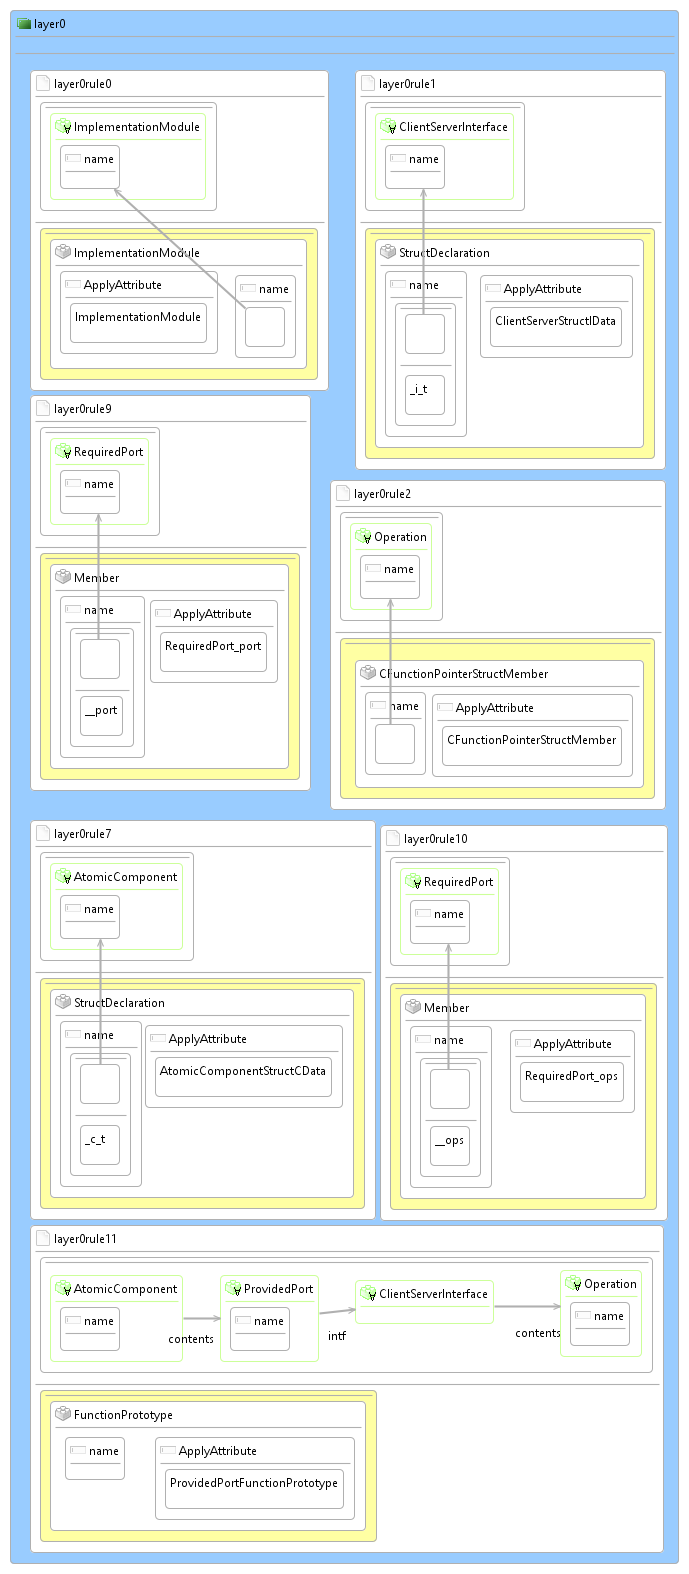
\includegraphics[width=0.48\textwidth]{figures/mbeddr2C_optimized_layer_0}
  \caption{Mbeddr-to-C transformation: layer 0.}
  \label{fig:mb2c_layer_0}
\end{center}
\end{figure}

% layer 1
\markus{Did we say anywhere that references between created nodes are
established in the next layer, relying on the traces?} In the second layer
(Layer 1) of the transformation, shown in Figure~\ref{fig:mb2c_layer_1}, the
previously created StructDeclaration elements are associated with the
ImplementationModule that was created in Layer 0 (Rule 0).
Also, in Rule 12 of this layer, the FunctionPrototype created in the Rule 11 of
the previous layer is associated with the ImplementationModule.
The other rules are similar.

\begin{figure}
\begin{center}
  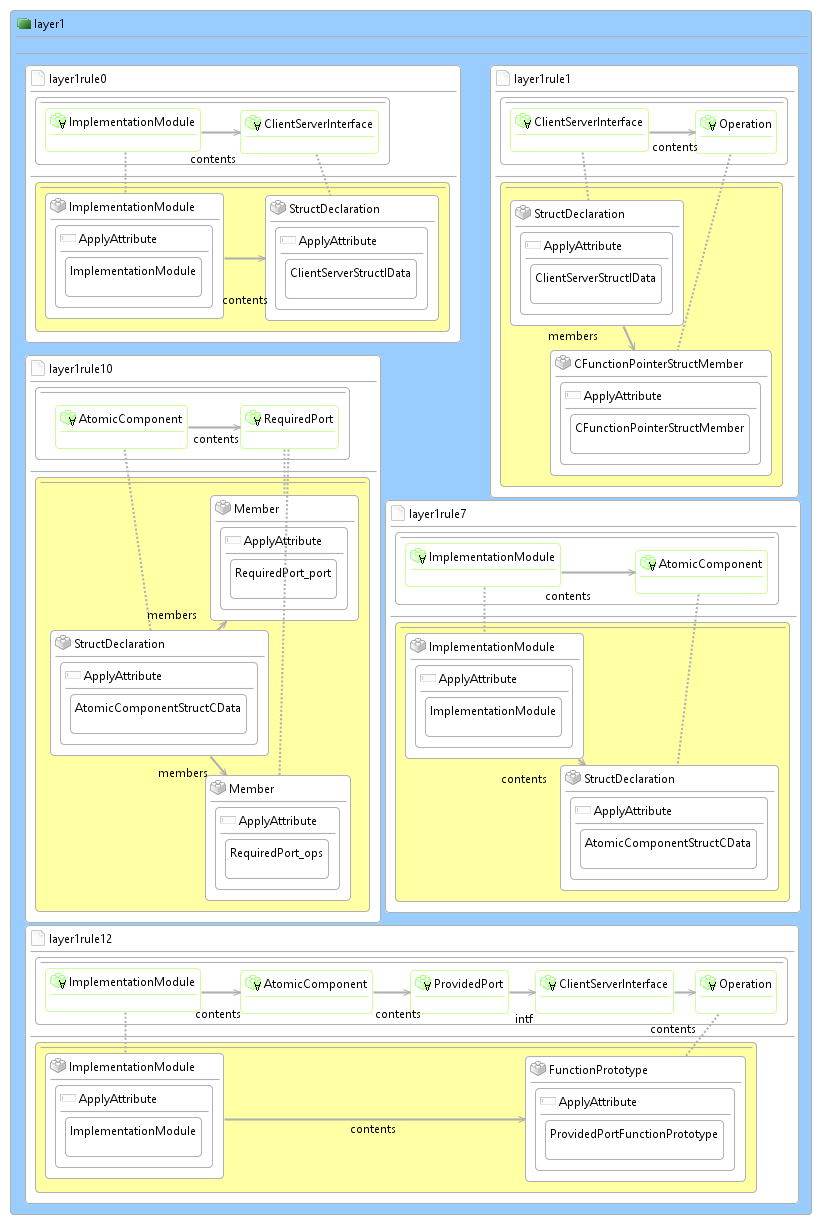
\includegraphics[width=0.48\textwidth]{figures/mbeddr2C_optimized_layer_1}
  \caption{Mbeddr-to-C transformation: layer 1.}
  \label{fig:mb2c_layer_1}
\end{center}
\end{figure}

% layer 3
In Layer 3, Figure~\ref{fig:mb2c_layer_3}, Rule 4 creates a
GlobalVariableDeclaration (ending in \verb=_inst=) for each ComponentInstance.
Rule 3 creates a GlobalVariableDeclaration for each ProvidedPort of each
ComponentInstance, ended in \verb=_ops=.
These variables will hold the the instance data of the component instance and
the address of the provided ports' operations of the component instance.

\begin{figure}
\begin{center}
  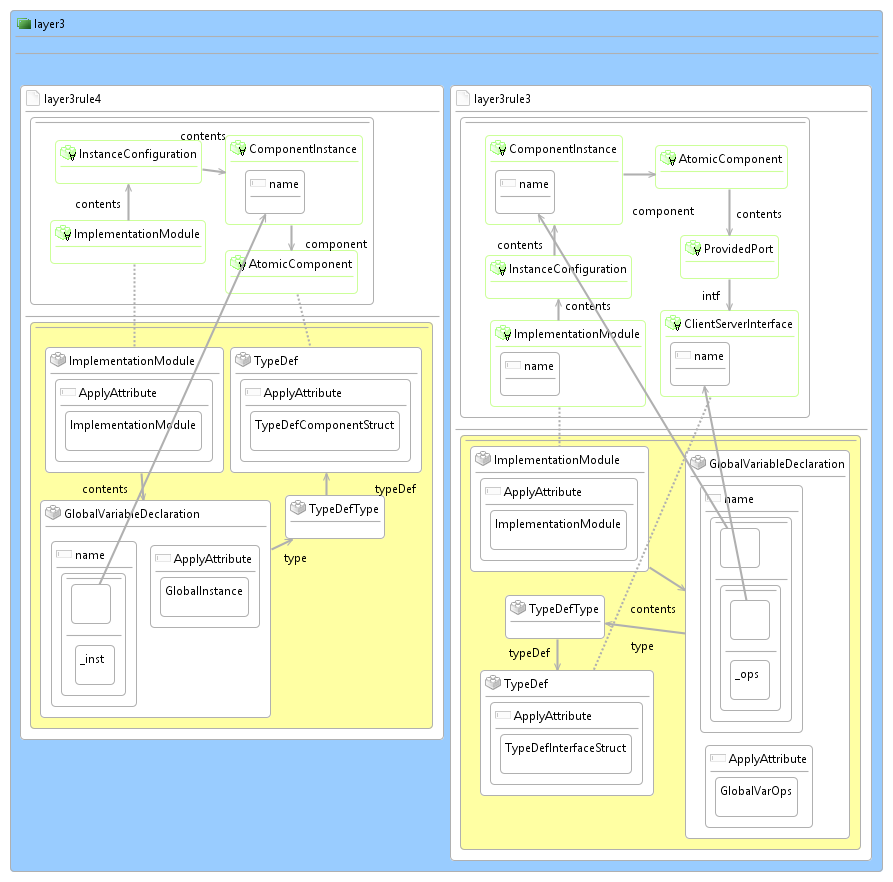
\includegraphics[width=0.48\textwidth]{figures/mbeddr2C_optimized_layer_3}
  \caption{Mbeddr-to-C transformation: layer 3.}
  \label{fig:mb2c_layer_3}
\end{center}
\end{figure}

% Layer 4
The next layer, Layer 4, Figure~\ref{fig:mb2c_layer_4}, creates the \verb=_wire=
(Rule 0) and \verb=init= (Rule 1) Functions from the ComponentInstances and the
InstanceConfiguration, respectively. These functions are created with an empty
body but they will later\markus{When, where, how?} implement the wiring of their
corresponding component instances. The \verb=init= function will just call all
the \verb=_wire= functions.

\begin{figure}
\begin{center}
  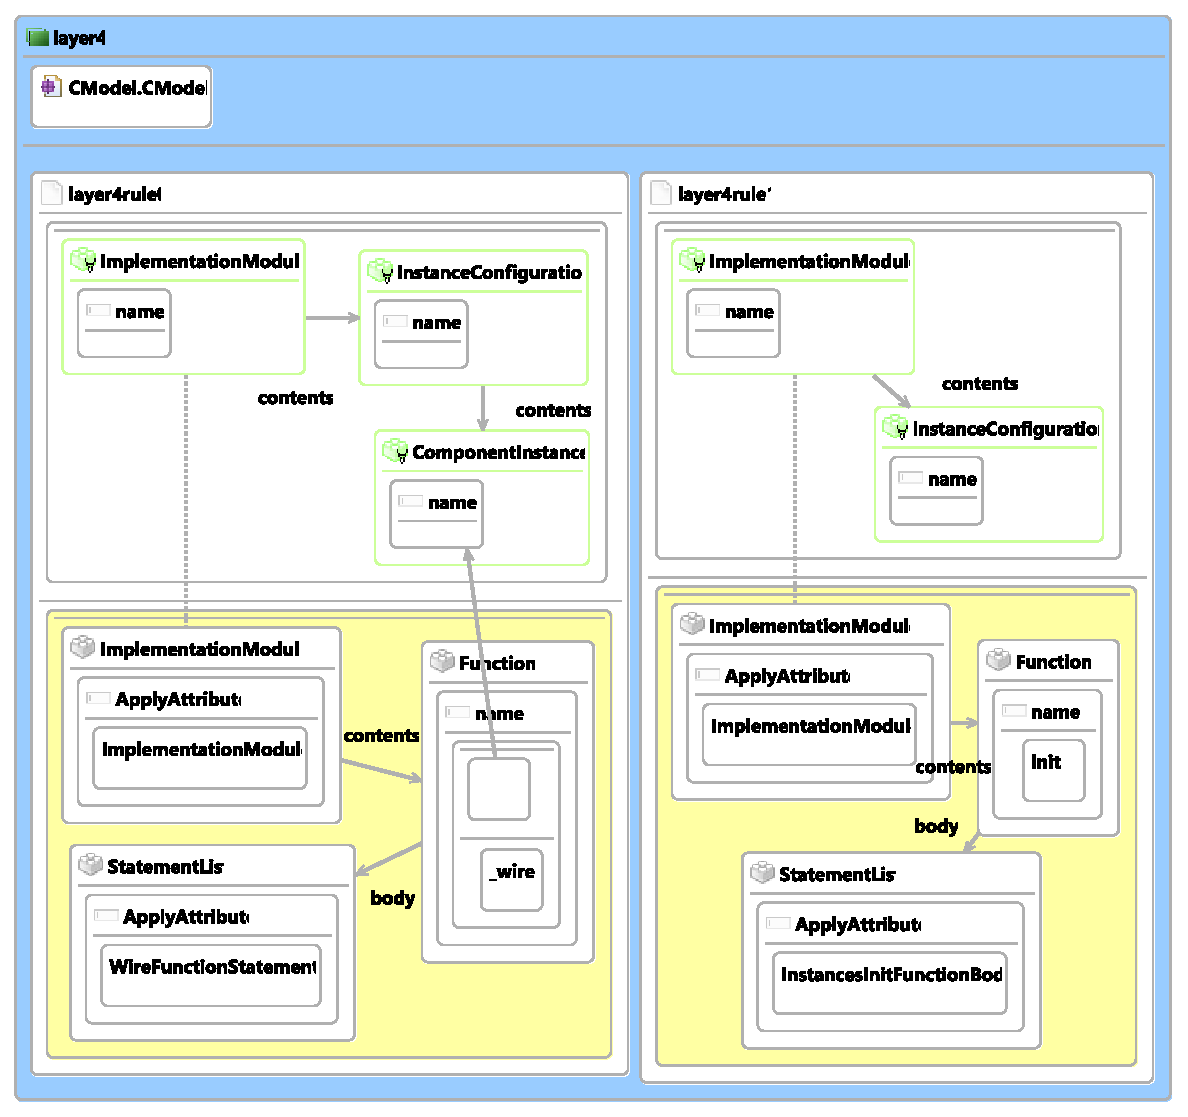
\includegraphics[width=0.48\textwidth]{figures/mbeddr2C_optimized_layer_4}
  \caption{Mbeddr-to-C transformation: layer 4.}
  \label{fig:mb2c_layer_4}
\end{center}
\end{figure}

% Layer 5
Finally, in the last layer, Layer 5, Figure~\ref{fig:mb2c_layer_5}, the bodies
of the \verb=init= and \verb=_wire= Functions are filled in.
Rule 0 adds an assignment to the \verb=_wire= Function body that assigns the
address of the function prototype created in Rule 11 of Layer 0, to the global
variable ended in \verb=_ops=, created in Layer 3, Rule 3.
This assignment does not connect a provided port with a required port:
it just saves the concrete function implementation in the \verb=_ops= variable.
The connection is made in Rule 1 of this layer. The match pattern is complex but
it essentially captures all the relevant entities that surround an
AssemblyConnector: the source and target component instances and their
provided/required ports. When a match for this rule is found, two assignments
are added to the \verb=_wire= function of the source component instance:
one to assign the address of the global variable that holds the instance data of
the target component instance; and one to assign the address of the variable
that holds the operations of the provided port to a member of the structure that
folds the required port operations of the source component instance.
Rule 2 is just adding to the body of the \verb=init=, a function call to each of
the \verb=_wire= functions.

\begin{figure}
\begin{center}
  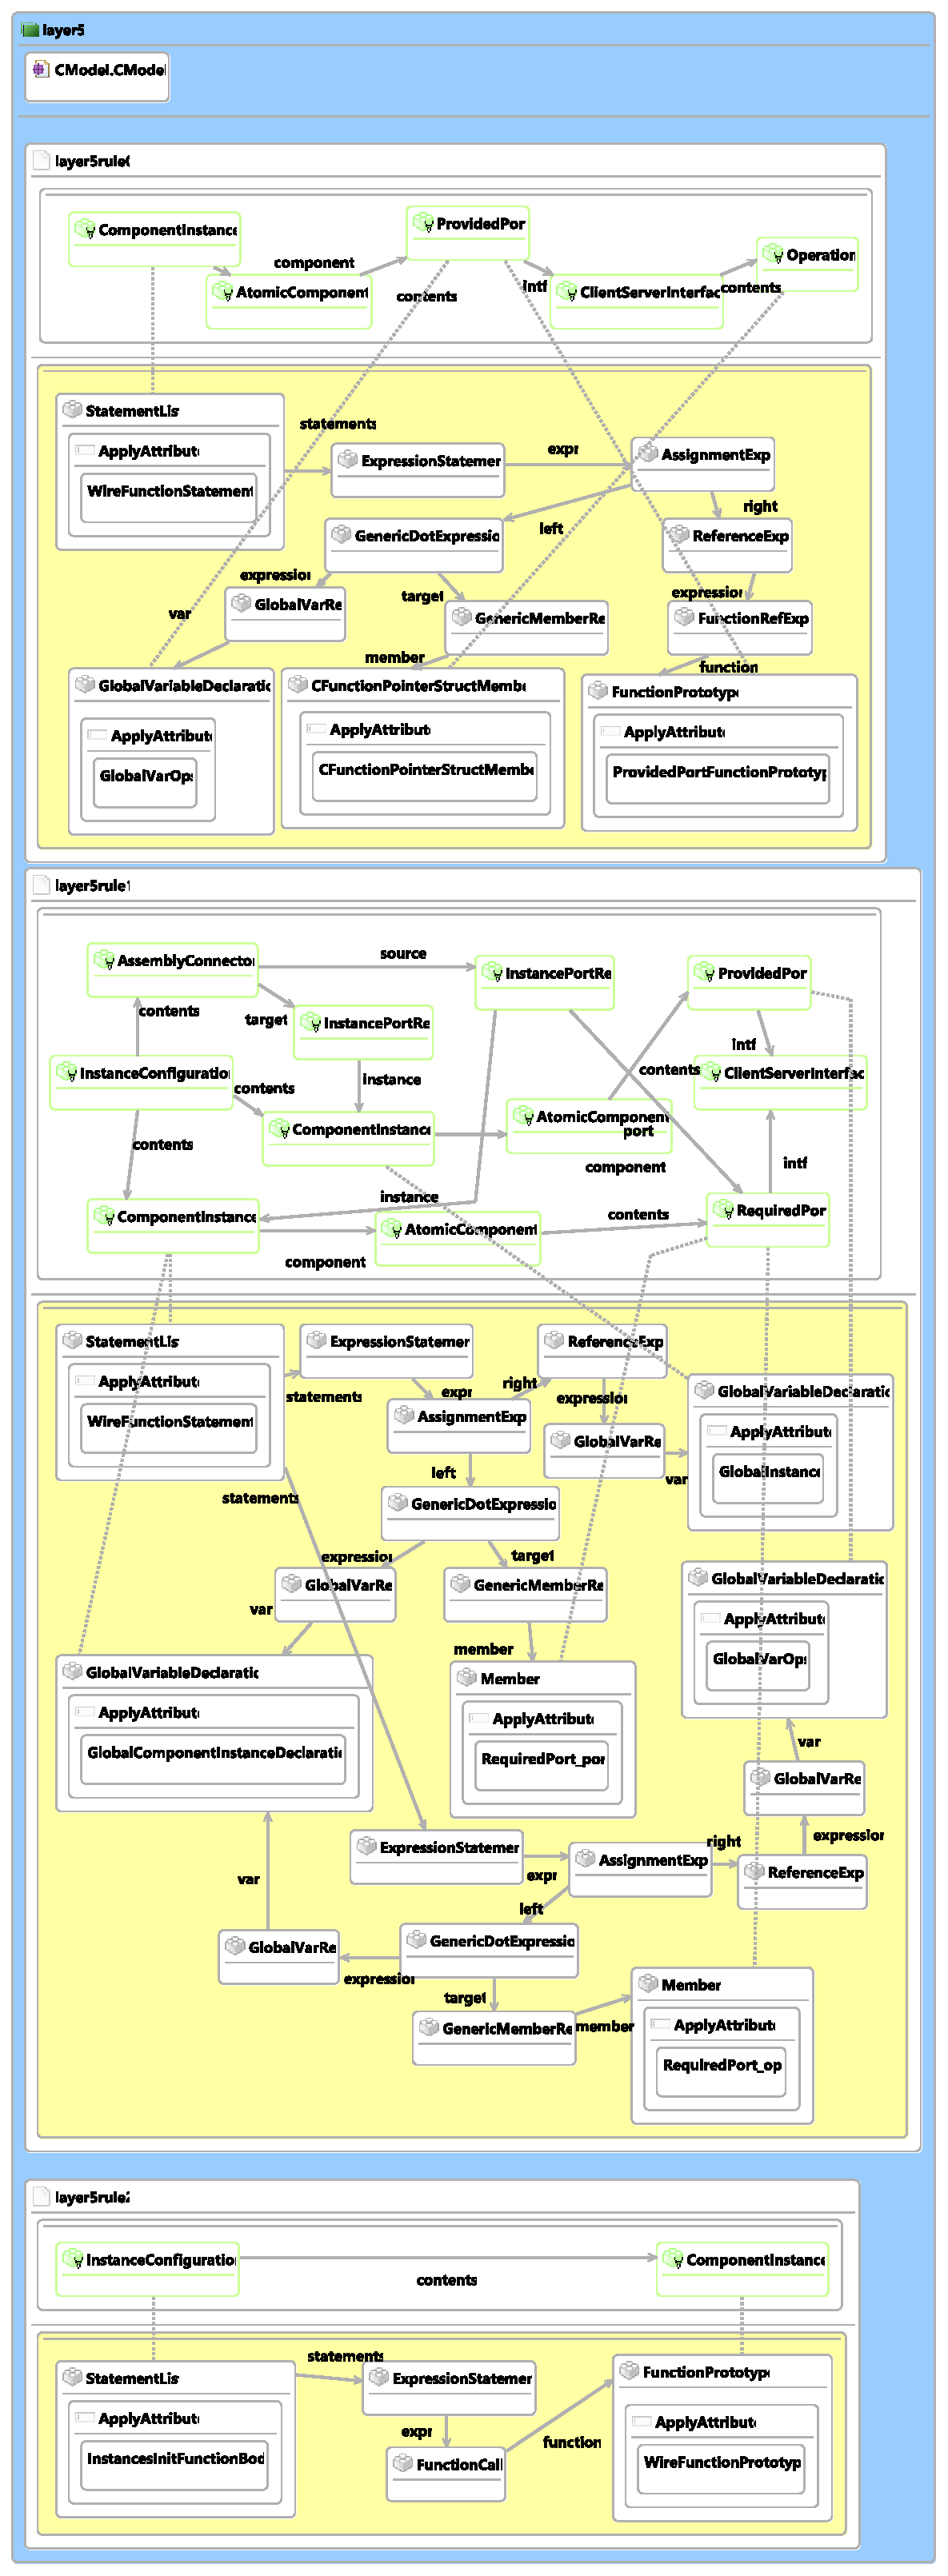
\includegraphics[width=0.48\textwidth]{figures/mbeddr2C_optimized_layer_5}
  \caption{Mbeddr-to-C transformation: layer 5.}
  \label{fig:mb2c_layer_5}
\end{center}
\end{figure}


\subsection{Correct Code Generation}

% pre-requisites for correctness.

In order for the transformation we just described to be correct, the wiring of
instances must be correct. The pre-requisites for this are:

\begin{compactenum}

\item The pointers to the provided port operations, assigned to the instance
variable that requires those operations do really point to the corresponding
operations.

\item The correct pointers are assigned to the correct instance variable.

\item Besides in the wiring function, that is called by the initialization
function, the instance variables' member that contains the provided port
operation reference is not assigned anywhere else.

\item The same thing as the previous for the pointers.
\end{compactenum}

\cgg{The above discussion is incomplete. I need to discuss this with Levi and Bentley and I need the SyVolt property.}























